\documentclass[11pt,a4paper]{article}
\usepackage[margin=0.85in]{geometry}
\usepackage{hyperref}
\usepackage{enumitem}
\usepackage{graphicx}
\usepackage{xcolor}
\usepackage{titling}
\usepackage{booktabs}
\usepackage{array}
\usepackage{tabularx}
\usepackage{float}
\usepackage{fancyhdr}
\hypersetup{colorlinks=true,linkcolor=blue,urlcolor=blue}
\pagestyle{fancy}
\fancyhf{}
\lhead{UCS503P -- Prototype Stage}
\rhead{Response Analysis Platform}
\cfoot{\thepage}
\setlength{\headheight}{14pt}
\setlength{\tabcolsep}{3pt}
\setlist[itemize]{leftmargin=0.7cm,itemsep=2pt,topsep=3pt}
\setlist[enumerate]{leftmargin=0.7cm,itemsep=2pt,topsep=3pt}
\newcommand{\BvrHint}[1]{{\normalfont\normalsize\itshape\hfill #1}}
\pretitle{\begin{center}\bfseries\fontsize{18bp}{20bp}\selectfont}
\posttitle{\par\end{center}\vskip 0.5em}

\title{AI Response Analysis and Prompt Engineering Platform}
\author{Keshav Batla\\Roll No.: \textit{[editable placeholder]}\\Email: \textit{[editable placeholder]}
  \and Diviyansh\\Roll No.: \textit{[editable placeholder]}\\Email: \textit{[editable placeholder]}
  \and Gurshant\\Roll No.: \textit{[editable placeholder]}\\Email: \textit{[editable placeholder]}}
\date{October 2026}

\begin{document}
\maketitle
\begin{center}
\large\textbf{Project Report -- Prototype Stage}\\[4pt]
Submitted for UCS503P -- Software Engineering Project\\
Thapar Institute of Engineering and Technology
\end{center}
\vspace{0.4em}
\noindent\textbf{Repository:}
\href{https://github.com/KeshavBatla/AI_RESPONSE-ANALYSIS_AND_PROMPT_ENGINEERING-PLATFORM}
{\texttt{AI Response Analysis and Prompt Engineering Platform}}

\section{Prototype objective \BvrHint{working vertical slice}}
The prototype demonstrates one complete user journey: enter a non-empty prompt,
generate a response through Google Gemini when the backend has a server-side API
key (or explicitly labelled deterministic demo text when demo mode is enabled),
and inspect five explained heuristic indicators. The platform does not train a
language model, persist interactions, or claim to reveal hidden reasoning.

\section{Problem and project requirements}
Users can receive answers that are unclear, long, incomplete, or poorly
formatted without a useful way to examine observable response characteristics.
The prototype integrates response generation with simple transparent signals
to support review; it is not a fact-checker or an objective quality oracle.

{\small
\noindent
\begin{tabularx}{\linewidth}{@{}>{\raggedright\arraybackslash}p{0.14\linewidth} X@{}}
\toprule
\textbf{ID} & \textbf{Requirement} \\
\midrule
FR-01 & Submit a non-empty prompt from a responsive browser interface. \\
FR-02 & Generate a live answer through the Google Gemini API using a backend-only environment key. \\
FR-03 & With no key, allow a deterministic response only when \texttt{DEMO\_MODE=true}, and label it as demo output. \\
FR-04 & Analyze a prompt/answer pair and return five integer scores (0--100) and at least one explanation. \\
FR-05 & Display the answer, five readable indicators, explanations, loading feedback, and useful errors. \\
FR-06 & Expose \texttt{GET /api/health}; reject empty generation and analysis inputs. \\
NFR-01 & Never send the provider key to the browser; restrict local CORS origins and bound provider timeouts. \\
NFR-02 & Keep analysis scores explicitly heuristic, not factuality or correctness guarantees. \\
NFR-03 & Do not claim prompt history is persisted; persistence is outside the prototype. \\
\bottomrule
\end{tabularx}
}

\section{Implemented architecture}
The React 18/Vite frontend (\path{Diviyansh/}) calls the FastAPI backend
(\path{KeshavBatla/backend_main.py}) using a configurable
\texttt{VITE\_API\_BASE\_URL}. At startup, the backend loads the repository-root
\path{.env} relative to its own source file. It uses Google's official
\texttt{google-genai} Python SDK Interactions API (default model
\texttt{gemini-3.8-flash}) for live generation with a server-only key, or
returns an explicitly labelled deterministic sample when demo mode is enabled
and no key is configured. Both generation and standalone analysis are API
endpoints. The shared heuristic analyzer remains in
\path{Gurshant/database_analysis.py}. The existing SQLAlchemy model definitions
are not connected to runtime operations; no database is required.

\begin{figure}[H]
\centering
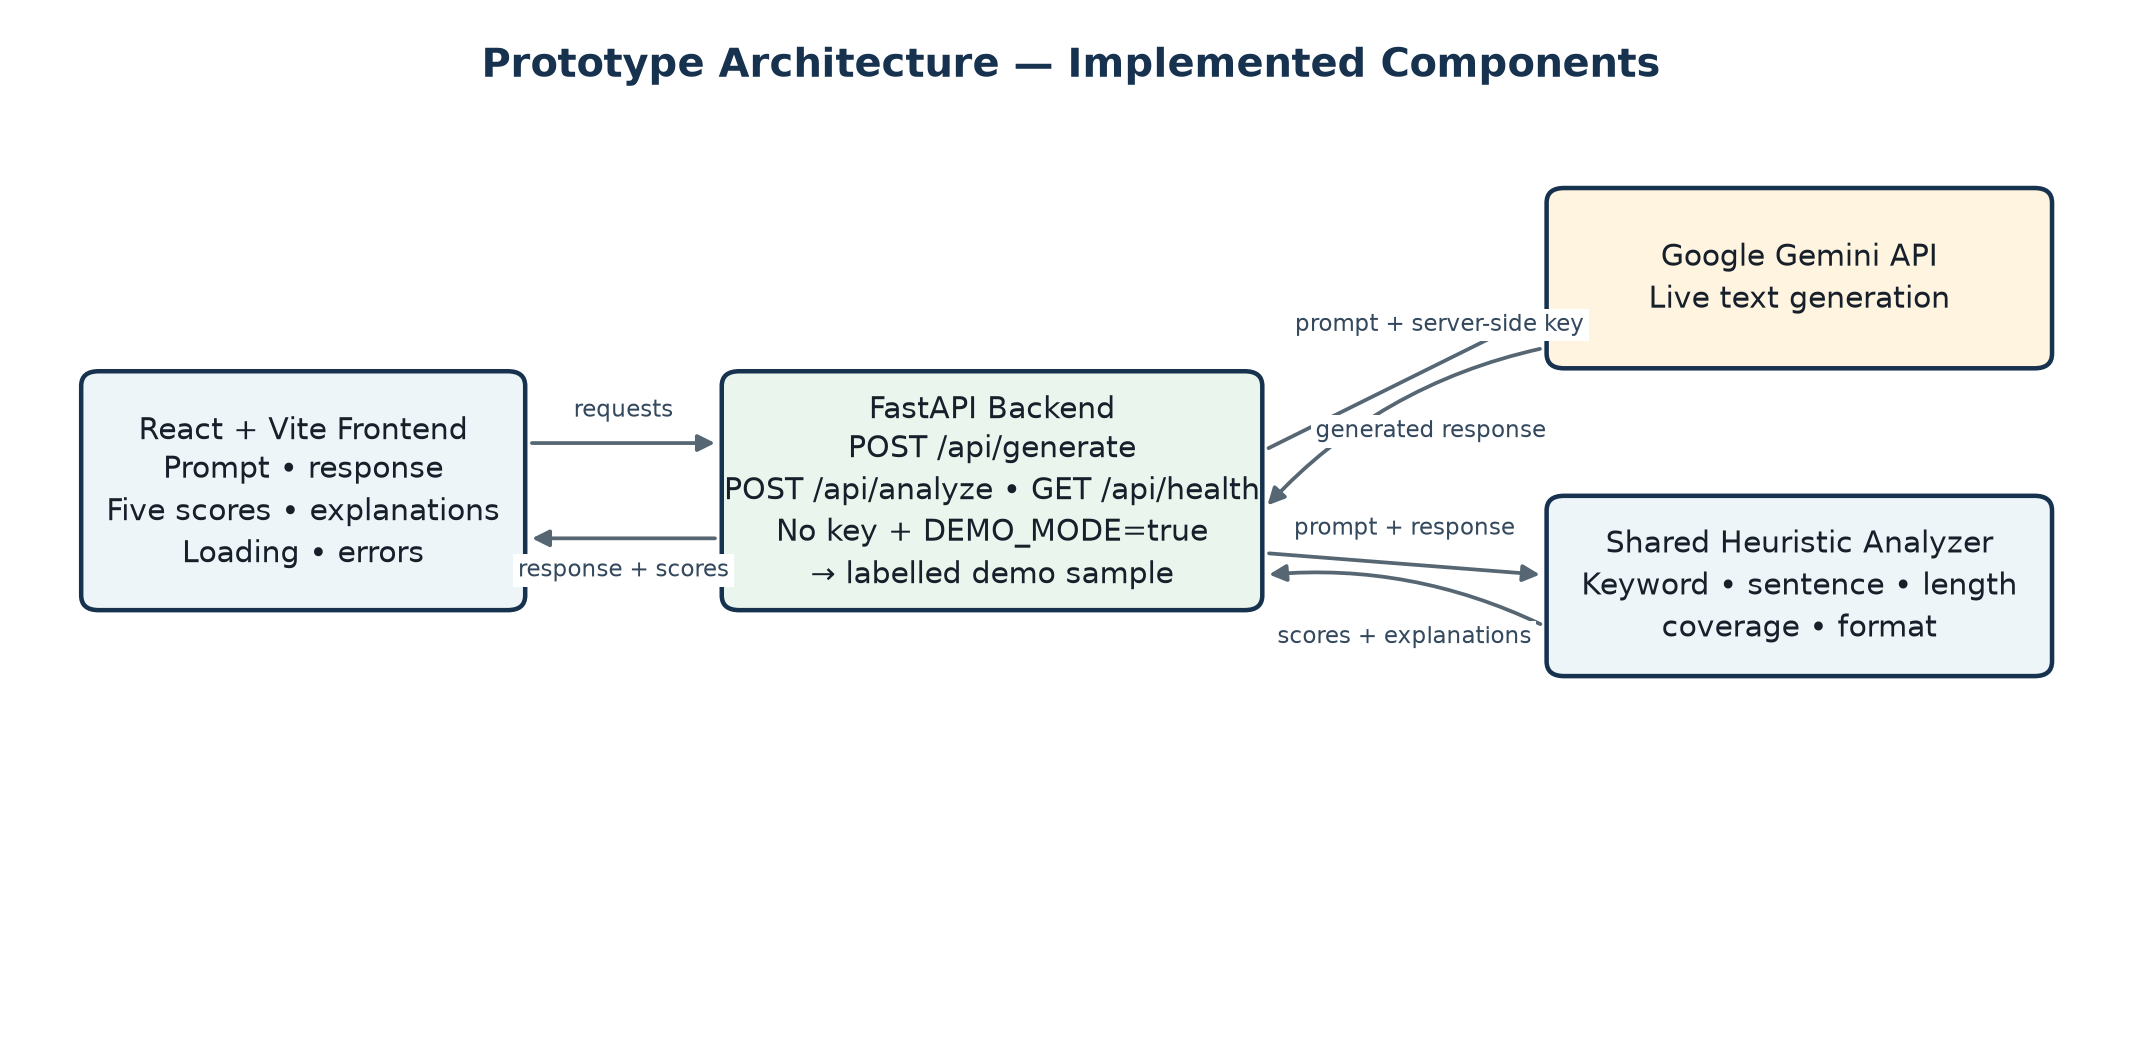
\includegraphics[width=0.96\linewidth]{assets/architecture.png}
\caption{Implemented frontend, API, shared analyzer, provider and labelled demo path.}
\end{figure}

\section{Data-flow diagrams}
\subsection{DFD Level 0 -- system context}
\begin{figure}[H]
\centering
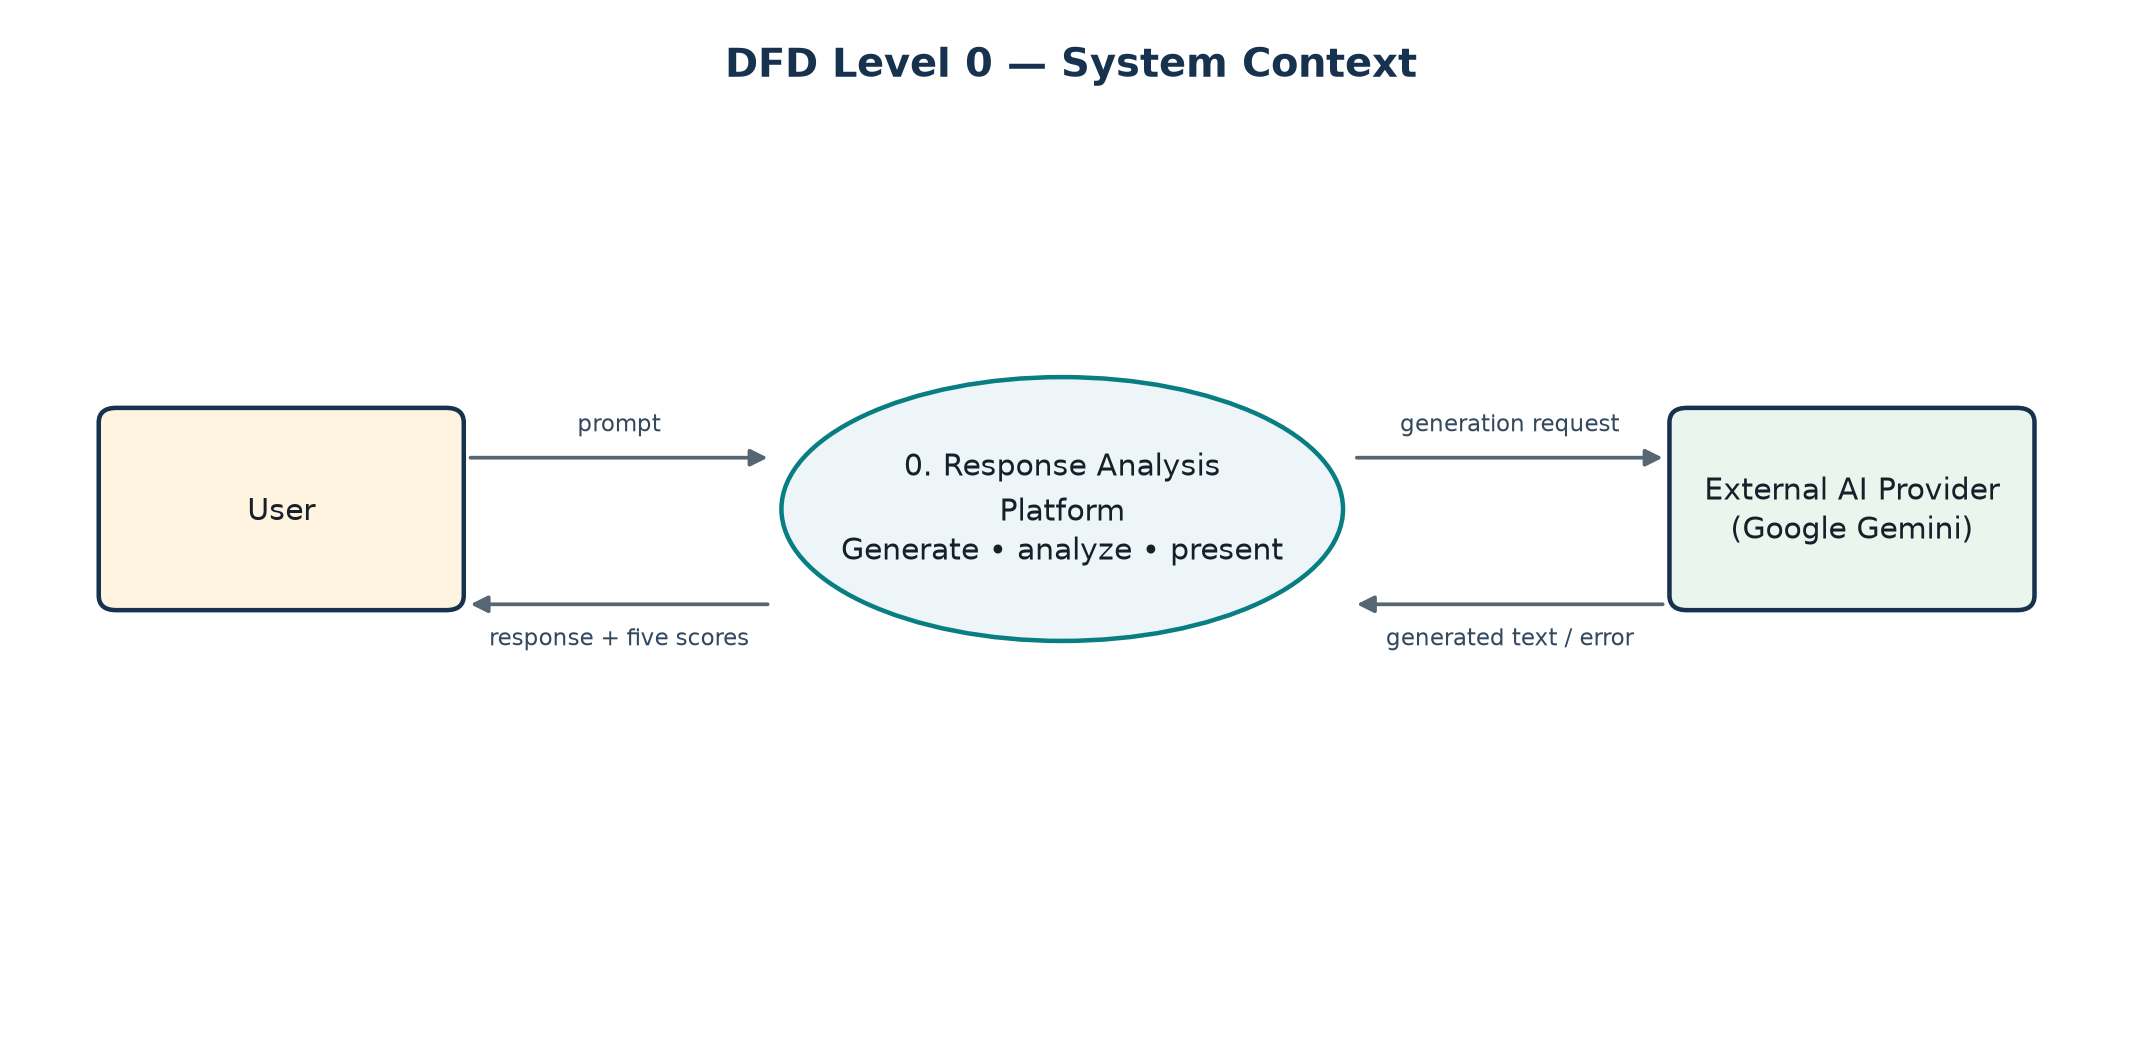
\includegraphics[width=0.94\linewidth]{assets/dfd_level0.png}
\caption{Prompt and evaluation exchange with the user; live generation with the external provider.}
\end{figure}

\subsection{DFD Level 1 -- processing detail}
\begin{figure}[H]
\centering
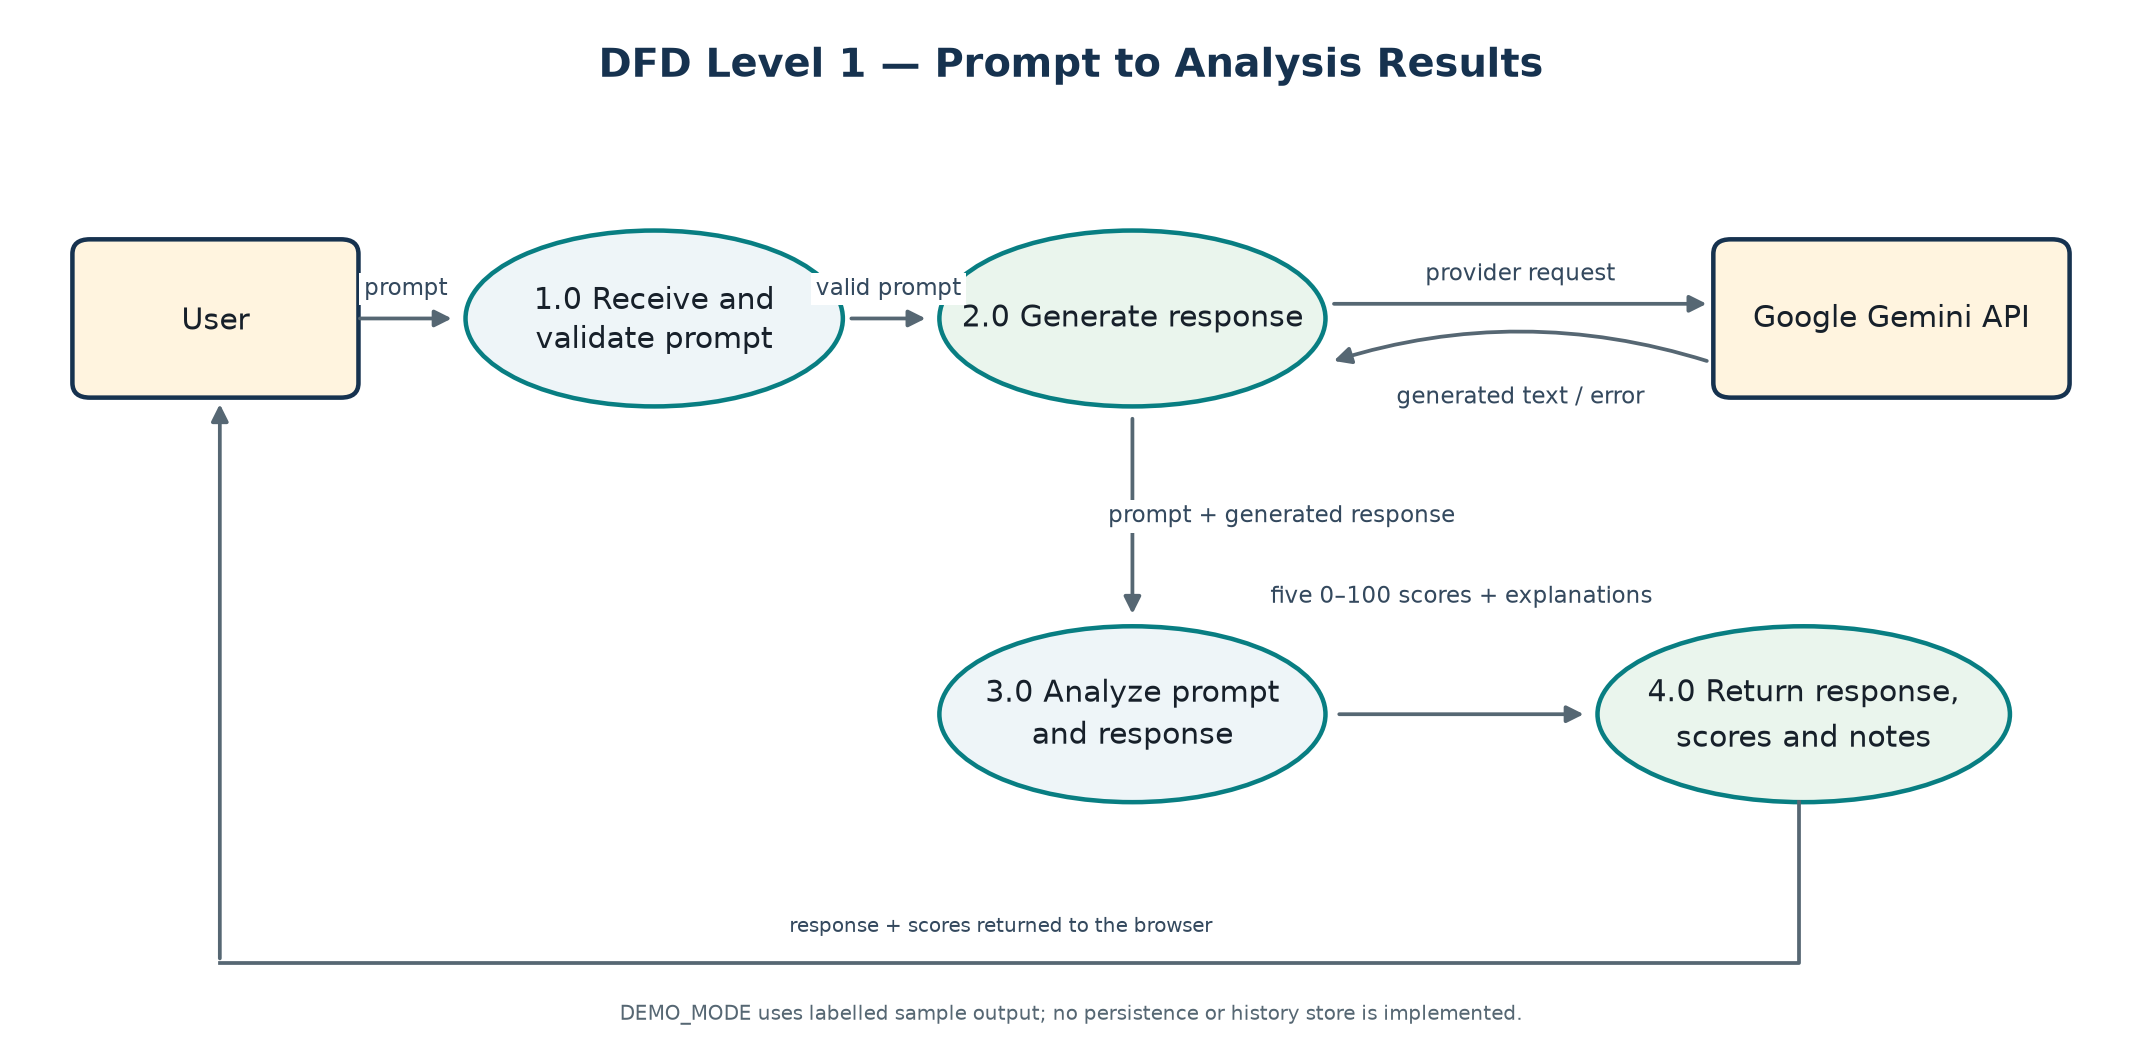
\includegraphics[width=0.96\linewidth]{assets/dfd_level1.png}
\caption{Prompt validation, response generation, heuristic analysis and browser results. No data store is implemented.}
\end{figure}

\section{Core workflow and interfaces}
\begin{enumerate}
  \item The user types a prompt or loads the sample prompt. The UI rejects an empty submission, shows a character count and prevents repeated submission while working.
  \item \texttt{POST /api/generate} validates the prompt. With \texttt{GEMINI\_API\_KEY}, the server calls the configured Gemini text model via the official SDK, with a finite 30-second timeout. Provider failures return a generic HTTP 502 response without exposing provider details.
  \item Without a key, generation returns HTTP 503 unless \texttt{DEMO\_MODE=true}. The deterministic response is marked \texttt{mode=demo}, names the deterministic model, and explicitly states that it was not generated by an AI model.
  \item After generation, the browser posts the same prompt and generated response to \texttt{POST} \path{/api/analyze}.
  \item The analyzer calculates relevance (keyword overlap), clarity (average sentence length), conciseness (word count), completeness (prompt-part coverage), and structure (formatting markers). Each score is clamped to 0--100 and accompanied by an observation.
  \item The UI displays the generated text, all five indicators, observation notes, and, for sample output, a persistent visible demo-mode banner.
\end{enumerate}

\section{Analysis method and limitations}
These inexpensive rule-based measures are inspectable proxies, not validated
judgements. Keyword overlap can miss paraphrases; sentence length is not the
same as comprehensibility; word count cannot determine whether content is
concise for its task; the comma/``and'' prompt split is a rough completeness
proxy; and formatting markers cannot establish logical organization. Scores
cannot establish factual correctness, safety, or model reasoning. Demo mode
illustrates wiring only and its sample is deliberately not presented as live AI
output. API keys must be supplied privately via environment variables; do not
commit a key or local environment file.

\section{Implementation status}
{\small
\noindent
\begin{tabularx}{\linewidth}{>{\raggedright\arraybackslash}p{0.25\linewidth} X}
\toprule
\textbf{Component} & \textbf{Status at this checkpoint} \\
\midrule
Prompt dashboard & Implemented React/Vite interface with sample prompt, responsive layout, request state, five score bars, explanations, and errors. \\
FastAPI & Implemented generation, analysis and health endpoints; input limits, restricted local CORS, environment-based provider configuration, bounded timeouts and sanitized provider errors. \\
Gemini integration & Implemented with the official \texttt{google-genai} SDK; live provider connectivity has not been exercised for this checkpoint. \\
Demo mode & Implemented; opt-in only, deterministic and labelled in API output, visible banner, and response content. \\
Heuristic analyzer & Integrated from the existing shared analysis module, validates empty inputs and clamps all five scores. \\
Tests & 15 unit and API tests pass. External generation is stubbed in the live-mode and error tests; no test issues a paid API request. \\
Persistence/history & Not implemented; interactions are not saved. SQLAlchemy models remain legacy definitions only. \\
Prompt optimization/comparison & Not implemented; future scope. \\
\bottomrule
\end{tabularx}
}

\section{Test cases and observed results}
Executed with \verb|.venv\Scripts\python.exe -m pytest -q|:
\textbf{16 passed, 2 warnings, 0 failed}. The warnings are Starlette's
deprecation notice about \texttt{httpx} in its test client and a Python 3.17
deprecation warning emitted by the installed Gemini SDK; neither failed tests.
No paid provider calls are made by the suite.

{\small
\noindent
\begin{tabularx}{\linewidth}{@{}>{\raggedright\arraybackslash}p{0.10\linewidth} >{\raggedright\arraybackslash}p{0.66\linewidth} >{\centering\arraybackslash}p{0.12\linewidth}@{}}
\toprule
\textbf{ID} & \textbf{Tested behaviour} & \textbf{Result} \\
\midrule
T-01 & Health route returns \texttt{\{"status":"ok"\}}. & Pass \\
T-02 & Blank generation prompt is rejected without a provider request. & Pass \\
T-03 & Blank prompt or response is rejected by analysis endpoint and analyzer. & Pass \\
T-04 & Analysis schema has exactly five bounded integer scores and explanations. & Pass \\
T-05 & Long unstructured response returns bounded scores and length feedback. & Pass \\
T-06 & Missing key without demo mode returns an explicit configuration error. & Pass \\
T-07 & Deterministic demo response is returned and explicitly labelled. & Pass \\
T-08 & Gemini SDK request, timeout configuration and text extraction use a stubbed client. & Pass \\
T-09 & Live generation route is tested using a stubbed provider; no external request. & Pass \\
T-10 & Stubbed provider failure returns generic error without sensitive detail. & Pass \\
\bottomrule
\end{tabularx}
}

\noindent The Vite production build completed successfully. A browser smoke test
also completed the demo-mode journey before the provider migration: the sample
prompt produced the labelled response, all five score cards and an explanation.
Live Gemini connectivity was not exercised for this checkpoint. No database or
persistence test is claimed.

\section{Risks and mitigations}
\begin{itemize}
  \item \textbf{Provider outage, invalid key or quota:} bounded outbound timeout, generic actionable error and a separately enabled demo path.
  \item \textbf{Gemini API/model availability:} the SDK marks the Interactions API experimental; access to the configured model is key-dependent and live connectivity has not been tested.
  \item \textbf{Secret exposure:} API key remains backend-only and comes from an environment variable; local \texttt{.env} files and keys are ignored by Git.
  \item \textbf{Misleading heuristic values:} label the five values as indicators, list their observable basis, and state that they are not factuality scores.
  \item \textbf{Data retention expectations:} interactions are not persisted; the UI and documentation do not promise history.
  \item \textbf{Local port conflicts:} use the documented API-base setting and allowed frontend origin if the default port is already occupied.
\end{itemize}

\section{Future plans}
\begin{enumerate}
  \item Evaluate and calibrate the heuristic indicators on human-reviewed prompt/response examples.
  \item Add optional, explicitly configured database persistence and user-visible history with appropriate retention controls.
  \item Add targeted prompt-improvement suggestions and revised-response comparison after the core analyzer is evaluated.
  \item Expand integration and accessibility checks; configure production deployment and security controls only after local prototype requirements are stable.
\end{enumerate}

\section{Team responsibilities}
\begin{itemize}
  \item \textbf{Keshav Batla -- Backend / AI integration:} FastAPI routes, Gemini SDK adapter, environment configuration and API error handling.
  \item \textbf{Diviyansh -- Frontend:} prompt dashboard, request state, score visualisation, explanations and responsive layout.
  \item \textbf{Gurshant -- Analysis / data layer:} transparent response-quality heuristics and existing SQLAlchemy model definitions.
\end{itemize}

\noindent\textbf{Student details:} roll numbers and email addresses are editable placeholders on the title page and must be filled in by the team.

\section{Conclusion}
The checkpoint delivers and tests the primary prompt-to-response-to-analysis
workflow with a Gemini integration path and a clearly marked no-key
demonstration path. The test suite passes locally and the frontend has a
production build. Live API behavior and persistence remain intentionally
unclaimed; heuristic scores remain interpretable but limited proxies.

\end{document}
